\documentclass[a4paper, 12pt, oneside]{article}
\usepackage[utf8]{inputenc}
\usepackage[margin=3cm, bindingoffset=1cm]{geometry}
\linespread{1.5}
\usepackage{float}
\usepackage{csquotes}
\usepackage{subfig}
\usepackage{graphicx}
\usepackage[table]{xcolor}
\usepackage{indentfirst}
\usepackage{fancyhdr}
\usepackage{alphabeta}
\usepackage{algpseudocode}
\usepackage{algorithm}
\usepackage{hyperref}
\usepackage[T1]{fontenc}
\usepackage{listings}
\usepackage[htt]{hyphenat}
\usepackage{pgfplots}
\usepackage{pgf-pie}
\usepackage[
    backend=biber,
    sorting=none
]{biblatex}
\addbibresource{bibliography.bib}


\setlength{\parindent}{1cm}

\pagestyle{fancy}
\fancyhf{}
\fancyhead[C]{\textbf{\leftmark}}
\fancyfoot[C]{\thepage}
\renewcommand{\headrulewidth}{1pt}
\renewcommand{\footrulewidth}{1pt}
\renewcommand{\contentsname}{Indice}

\usepackage[Conny]{fncychap}

  
\begin{document}
\begin{titlepage}
    \begin{center}
        \LARGE{\uppercase{Università degli Studi di Salerno}}\\
        \vspace{5mm}
    	\uppercase{\normalsize Dipartimento di Informatica }\\
    \end{center}
    \begin{figure}[H]
        \centering
        
\includegraphics[width=0.35\textwidth]{logo_unisa}
    \end{figure}
    
    \begin{center}
        \normalsize{Corso di \textbf{Penetration Testing and Ethical Hacking}}\\
    	\vspace{10mm}
    	\LARGE{\textbf{\textsc{NoobBox-1}:\\ Penetration Testing Report}}\\
    	\vspace{3mm}
        \large{\uppercase{Anno Accademico 2022/2023}}
    \end{center}

    \vspace{70mm}
    \noindent
    \begin{minipage}[t]{0.6\textwidth}
    	Docente:\\\textbf{Prof. Arcangelo Castiglione}
    	\vspace{10mm}\\
    \end{minipage}
    \hfill
    \begin{minipage}[t]{0.4\textwidth}\raggedleft
    	Studente: \\\textbf{Hermann Senatore}
    \end{minipage}
\end{titlepage}

\tableofcontents
\newpage

\section{Scopi e struttura del documento}

Il \textbf{Penetration Testing Report} consiste in un resoconto, articolato in diversi livelli di dettaglio, sulle varie fasi del processo di Penetration Testing condotto sull'asset.

Tale documento è articolato in diverse sezioni. Ciascuna di queste si concentra su aspetti diversi. In particolare:

\begin{enumerate}
    \item \textbf{Executive Summary}: in questa sezione viene svolta una sintesi dei risultati del processo e dello stato generale di sicurezza del sistema analizzato;
    \item \textbf{Engagement Highlights}: in questa sezione vengono esplicitate le regole di ingaggio tra chi ha commissionato l'indagine ed il Penetration Tester, le metodologie e gli obiettivi dell'analisi;
    \item \textbf{Vulnerability Report}: in questa sezione viene fornita una visione d'insieme delle problematiche di sicurezza di cui l'asset è affetto;
    \item \textbf{Findings Summary}: in questa sezione vengono presentate con maggior livello di dettaglio le vulnerabilità riscontrate durante il processo di Penetration Testing;
    \item \textbf{Remediation Report}: in questa sezione sono proposte eventuali soluzioni alle vulnerabilità ed alle debolezze descritte nella sezione precedente;
    \item \textbf{Detailed Summary}: in questa sezione è presente una discussione approfondita sulle problematiche individuate in precedenza.
\end{enumerate}

\newpage
\section{Executive Summary}
Il processo di Penetration Testing che questo documento sommarizza è stato svolto su un asset \textit{vulnerable by default} denominato \textbf{NoobBox-1} reperibile presso la piattaforma \textbf{VulnHub} all'indirizzo \url{https://www.vulnhub.com/entry/noobbox-1,664/}. Nato come sfida CTF, è stato utilizzato dall'autore del presente documento per prendere confidenza con i tool e le metodologie più utilizzate nel contesto del Penetration Testing.

Gli obiettivi che sono stati fissati e raggiunti in questo processo consistono sostanzialmente in:

\begin{itemize}
    \item Identificazione ed enumerazione completa dei servizi presenti all'interno dell'asset;
    \item Rilevamento delle vulnerabilità e delle debolezze presenti all'interno dell'asset;
    \item Ottenere accesso privilegiato alla macchina;
    \item Provvedere all'installazione di software specializzato per permettere l'accesso persistente all'asset.
\end{itemize}

L'attività di Penetration Testing è stata condotta a partire dal giorno 22 maggio 2023 ed ha avuto una connotazione \textbf{grey box} poiché alcune informazioni sono reperibili direttamente dalla piattaforma VulnHub e che fungono da punto di partenza.

Il livello di rischio derivato dall'analisi è stato classificato come \textbf{Medio-Alto} perché sebbene non siano presenti vulnerabilità intrinseche dei servizi in esecuzione che siano direttamente sfruttabili, è stato comunque possibile ottenere accesso privilegiato alla macchina mediante \textbf{errori di configurazione} e pratiche di sicurezza \textbf{scorrette}.

Una volta applicate le migliorie e le correzioni descritte nella sezione denominata \textbf{Remediation Report}, il livello di rischio scenderebbe ad un livello tale da non permettere più l'accesso non autorizzato alla macchina.

\newpage

\section{Engagement Highlights}
Poiché l'analisi descritta da questo documento consiste in un progetto di stampo accademico e l'asset considerato ha questo tipo di analisi come scopo dichiarato, non sono state definite delle limitazioni dal punto di vista legale o contrattuale. 

In particolare, non sono presenti parti dell'asset che non sarebbero dovute essere analizzate così come non è stata imposta alcuna limitazione riguardo gli strumenti da utilizzare. 

Inoltre, non è stato (ovviamente) previsto alcun accordo di non-divulgazione.

\newpage

\section{Vulnerability Report}
\label{sec:vulnrep}
In questa sezione viene proposta un'\textit{overview} delle problematiche di sicurezza presenti sull'asset.

In particolare, le problematiche appartengono alle categorie di:

\begin{itemize}
    \item Information disclosure;
    \item Obsolescenza del software utilizzato dall'asset;
    \item Errori di configurazione e cattive pratiche di sicurezza;
\end{itemize}

\subsection{Information Disclosure}
Alcune informazioni sensibili che possono essere ricollegate a meccanismi di funzionamento interni all'asset sono \textbf{pubblicamente accessibili}. In particolare, visitando il sito web offerto dall'asset all'URL \texttt{/img.jpg} è possibile rinvenire la password dell'utente amministratore di \textbf{Wordpress}. Inoltre, lo username di quest'ultimo è enumerabile mediante scansioni automatiche. Entrambi questi aspetti consentono immediatamente l'accesso non autorizzato all'asset.

\subsection{Obsolescenza del software utilizzato nell'asset}
Alcune componenti dell'asset sono ormai \textbf{obsolete}. In particolare, il server web \textbf{Apache httpd} è aggiornato alla versione \textbf{2.4.38}, rilasciata il \textbf{22 gennaio 2019}. Questa versione del software risulta essere afflitta da alcune vulnerabilita. Sebbene nessuna di queste sia risultata sfruttabile per ottenere l'accesso alla macchina, l'obsolescenza dei software, sia nel caso di \texttt{httpd2} che di qualunque altro software rende sempre più probabile la compromissione dell'asset man mano che passa il tempo.

\subsection{Cattive pratiche di sicurezza}
L'utente della macchina locale possiede \textbf{lo stesso username} dell'utente che amministra il sito web creato con \textbf{Wordpress}. Una situazione del genere semplifica notevolmente il processo di enumerazione dell'asset, che può condurre alla sua compromissione. A peggiorare la situazione è stata la constatazione di un \textbf{riuso} della password per i due account. Una situazione del genere consente ad un attaccante di accedere ai file personali dell'utente locale dell'asset. 

È stata inoltre rilevata la possibilità per l'utente locale di eseguire software con privilegi \textbf{ingiustamente elevati}. Quest'ultimo aspetto, in caso di accesso non autorizzato, permette di effettuare \textbf{Privilege Escalation}.

\newpage
\section{Findings Summary}
In questa sezione viene proposta una panoramica dei risultati della fase di \textbf{Vulnerability Assessment}, che si propone di rilevare le vulnerabilità di cui l'asset è affetto. Siccome per eseguire la ricerca delle vulnerabilità è stato utilizzato più di un tool, il conto delle vulnerabilità non includerà più volte una vulnerabilità già riscontrata una volta. Il totale tra vulnerabilità riscontrate ed informazioni ammonta a \textbf{53}. Nessuna delle vulnerabilità di livello alto si è rivelata sfruttabile.

Seguono dei diagrammi che forniscono una più chiara ripartizione dei rilevamenti.

\vspace{15mm}
    \begin{table}[h!]
        \centering
        \begin{tabular}{|l|l|l|l|l|}
            \hline
            Livello di Rischio                              & \cellcolor[HTML]{FE0000}HIGH & \cellcolor[HTML]{FFCC67}MEDIUM & \cellcolor[HTML]{34FF34}LOW & \cellcolor[HTML]{34CDF9}INFO \\ \hline
            \multicolumn{1}{|c|}{\textit{\# vulnerabilità}} & \multicolumn{1}{c|}{20}      & \multicolumn{1}{c|}{14}        & \multicolumn{1}{c|}{2}      & \multicolumn{1}{c|}{17}      \\ \hline
        \end{tabular}
    \end{table}
    \vspace{15mm}
    \begin{center}
        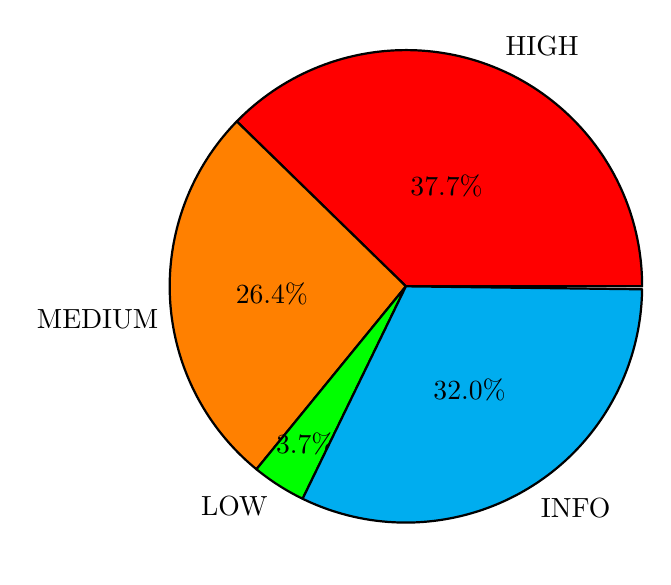
\begin{tikzpicture}
            \pie[color={red!100,orange!100,green!100,cyan!100}]{37.7/HIGH, 26.4/MEDIUM, 3.7/LOW, 32.0/INFO}
        \end{tikzpicture}
    \end{center}
        
\newpage

\section{Remediation Report}
In questa sezione verranno presentate delle strategie per risolvere o mitigare le problematiche di sicurezza emerse durante il processo svolto e documentate nella \hyperref[sec:vulnrep]{Sezione 4}.

\subsection{Remediation per \textbf{Information Disclosure}}
\begin{enumerate}
    \item \textbf{Eliminare} il file \texttt{img.jpg} dalla root del web server per evitare di divulgare la password dell'amministratore di \textbf{Wordpress};
    \item Installare e configurare il plugin di Wordpress \textbf{Stop User Enumeration} per contrastare tool di enumerazione automatica \cite{sue};
    \item Aggiornare il profilo dell'amministratore di \textbf{Wordpress} ed utilizzare un \textbf{Display Name} diverso dallo username.
\end{enumerate}

\subsection{Remediation per \textbf{Obsolescenza del software}}
La strategia più semplice (ma anche la migliore!) per risolvere le criticità appartenenti a questa categoria consiste nell'applicare in maniera frequente le \textbf{patch dei vendor} dei vari software in esecuzione, con una particolare attenzione ad \textbf{Apache httpd}. Tale processo può essere svolto sia \textbf{manualmente} che \textbf{automaticamente}, utilizzando sistemi di scheduling dei task come ad esempio \texttt{cron} nei momenti in cui tipicamente il traffico verso il sito web è minore.

\newpage
\subsection{Remediation per \textbf{Cattive pratiche di sicurezza}}
\begin{enumerate}
    \item Modificare lo username dell'utente della macchina locale (o quello dell'admin di Wordpress) per far sì che non siano identici e contrastare il processo di enumerazione;
    \item Ripetere lo stesso procedimento descritto al punto precedente per le \textbf{password} dei due account;
    \item Eliminare dal file \texttt{/etc/sudoers} la possibilità per l'utente \texttt{noobbox} di eseguire il comando \texttt{vim} come utente \texttt{root}.
\end{enumerate}
\newpage

\section{Detailed Summary}
In questa sezione vengono fornite informazioni dettagliate sulle vulnerabilità e sulle debolezze di cui l'asset è affetto che sono state riscontrate durante il processo di Penetration Testing nella fase di \textbf{Vulnerability Mapping}.

Per assolvere a tale compito, sono stati utilizzati in particolare tre tools:

\begin{enumerate}
    \item \textbf{Nessus};
    \item \textbf{OpenVAS};
    \item \textbf{LinPEAS}, utilizzato per ottenere informazioni utili alla \textbf{Privilege Escalation} ma che ha permesso di rilevare vulnerabilità che affliggono, tra gli altri, il tool \texttt{sudo}.
\end{enumerate}

\subsection{Nessus}
Un resoconto dettagliato delle vulnerabilità rilevate dal tool \textbf{Nessus} è allegato al presente documento ed è presente al percorso \texttt{extra/Nessus-Scan.pdf}. Si noti che tale tool ha prodotto \textbf{due falsi positivi}, di cui è stato discusso nella documentazione del processo. In particolare, le vulnerabilità etichettate come:

\begin{itemize}
    \item 42423 - CGI Generic SSI Injection (HTTP headers);
    \item 57640 - Web Application Information Disclosure 
\end{itemize}

sono falsi positivi e come tali \textbf{non sono stati considerati nel conteggio finale delle vulnerabilità}

\subsection{OpenVAS}
Parimenti, un resoconto dettagliato delle vulnerabilità rilevate dal tool \textbf{OpenVAS} è allegato al presente documento ed è presente al percorso \texttt{extra/OpenVAS-Scan.pdf}.

\subsection{LinPEAS}
Poiché tale tool non fornisce un output strutturato, sono di seguito riportate informazioni dettagliate sulla natura delle vulnerabilità rilevate.

\subsubsection{CVE-2019-13272}
\begin{itemize}
    \item \textbf{Descrizione:} nelle versioni del Kernel Linux precedenti alla 5.1.17, la funzione \texttt{ptrace\_link()} all'interno del file \texttt{kernel/ptrace.c} gestisce male le credenziali di un processo che intende sfruttare il meccanismo delle relazioni \texttt{ptrace}. In determinati scenari, tipicamente quando sussiste una relazione padre-figlio, la situazione potrebbe essere sfruttata da un utente locale per ottenere \textbf{accesso root}.
    \item \textbf{Livello di Impatto}: HIGH;
    \item \textbf{Punteggio CVSS v3}: 7.8;
    \item \textbf{Riferimento}: \cite{13272}
    \item \textbf{Contromisura}: effettuare un aggiornamento software, in particolare del \textbf{kernel}.
\end{itemize}

\subsubsection{CVE-2019-18634}
\begin{itemize}
    \item \textbf{Descrizione:} nelle versioni di \texttt{sudo} precedenti alla 1.8.26, l'opzione \texttt{pwfeedback} (utilizzata per far apparire degli asterischi mentre si sta digitando la password ad un prompt di \texttt{sudo}) attivabile all'interno del file \texttt{/etc/sudoers} permetteva ad un attaccante di veicolare un attacco di \textbf{stack based buffer overflow} mediante l'utilizzo di una stringa di caratteri molto lunga.
    \item \textbf{Livello di Impatto}: HIGH;
    \item \textbf{Punteggio CVSS v3}: 7.8;
    \item \textbf{Riferimento}: \cite{18634}
    \item \textbf{Contromisura}: effettuare un aggiornamento software, in particolare del pacchetto \textbf{sudo}.
\end{itemize}

\subsubsection{CVE-2021-22555}
\begin{itemize}
    \item \textbf{Descrizione:} nelle versioni del Kernel Linux a partire dalla 2.6.19-rc1 è stato rilevato un \textbf{heap-out-of-bound write} nel file \texttt{net/netfilter/x\_tables.c}, tramite il quale è possibile veicolare un attacco di \textbf{Denial of Service} usando la tecnica dell'\textbf{heap based memory corruption}. 
    \item \textbf{Livello di Impatto}: HIGH;
    \item \textbf{Punteggio CVSS v3}: 7.8;
    \item \textbf{Riferimento}: \cite{22555}
    \item \textbf{Contromisura}: effettuare un aggiornamento software, in particolare del \textbf{kernel}.
\end{itemize}
\newpage

\subsection{Altre debolezze e criticità}
Oltre alle vulnerabilità rilevate dai tool prima menzionati, l'asset è affetto da ulteriori debolezze ed errori di configurazione che possono portare ad accessi non autorizzati e \textbf{privilege escalation}.

\subsubsection{Disclosure della password di Wordpress}
\begin{itemize}
    \item \textbf{Descrizione}: alla pagina \texttt{http://192.168.64.21/img.jpg} è possibile visualizzare una password che può essere ricondotta facilmente a quella dell'amministratore di wordpress;
    \item \textbf{Rischi e potenziali attacchi}: in combinazione con la debolezza che riguarda l'enumerabilità degli utenti di Wordpress già rilevata da \textbf{Nessus}, tale debolezza può essere utilizzata per impersonare l'amministratore di \textbf{Wordpress};
    \item \textbf{Contromisura}: eliminare il file \texttt{img.jpg} dal web server.
\end{itemize}

\subsubsection{Riuso degli username e delle password}
\begin{itemize}
    \item \textbf{Descrizione}: sia l'utente locale dell'asset che l'admin di Wordpress condividono la stessa coppia di credenziali.
    \item \textbf{Rischi e potenziali attacchi}: nel caso un attaccante riesca ad entrare in possesso delle credenziali di un account, ha automaticamente compresso anche l'altro;
    \item \textbf{Contromisura}: cambiare nome utente e password ad uno dei due account.
\end{itemize}

\subsubsection{Esecuzione di \texttt{vim} come root}
\begin{itemize}
    \item \textbf{Descrizione}: tale politica di sicurezza scorretta è stata rilevata sia manualmente andando ad analizzare il file \texttt{/etc/sudoers} che mediante \textbf{LinPEAS}. La configurazione corrente del tool \texttt{sudo} non permette all'utente \texttt{noobbox} di eseguire alcun comando come root, ad eccezione del comando \texttt{vim}. Anche in questo modo è comunque possibile ottenere una shell di root.
    \item \textbf{Rischi e potenziali attacchi}: l'esecuzione dell'editor \texttt{vim} supporta l'esecuzione di un "comando" dell'editor subito dopo il suo avvio. Mediante il comando \texttt{vim -c ':!<cmd>'} è possibile eseguire il comando di shell \texttt{<cmd>} all'apertura dell'editor. Usando \texttt{sudo vim -c ':!/bin/bash'} viene aperta una \textbf{shell di root}.
    \item \textbf{Contromisura}: inibire anche l'accesso al comando \texttt{vim} andando a modificare il file \texttt{/etc/sudoers} ed eliminare le righe che recitano: \begin{center}
        \texttt{User noobbox may run the following commands on N00bBox:\\
    (ALL : ALL) /usr/bin/vim}
    \end{center}
\end{itemize}
\newpage
\printbibliography[title={Riferimenti bibliografici}]
\end{document}